\documentclass[11pt]{article}
\usepackage[margin=2cm]{geometry}
\usepackage{graphicx}
\usepackage{amsmath,amssymb}
\setlength{\parindent}{0pt}\setlength{\parskip}{5pt}
\graphicspath{{figures/}}
\begin{document}
\begin{center}{\Large\bfseries s9\_np (fixed target) --- Figure Notes for the Defense}\\[2pt]
5 deterministic episodes, gate 0.03~m / 2.9$^\circ$, 5/5 success ($=100\%$); mean min $d$ = 0.0258~m, mean min $\varphi$ = 1.4$^\circ$. Date 2026-09-24.\end{center}
\vspace{4pt}
\section*{Figure 1 --- Reach: distance to target}
\begin{center}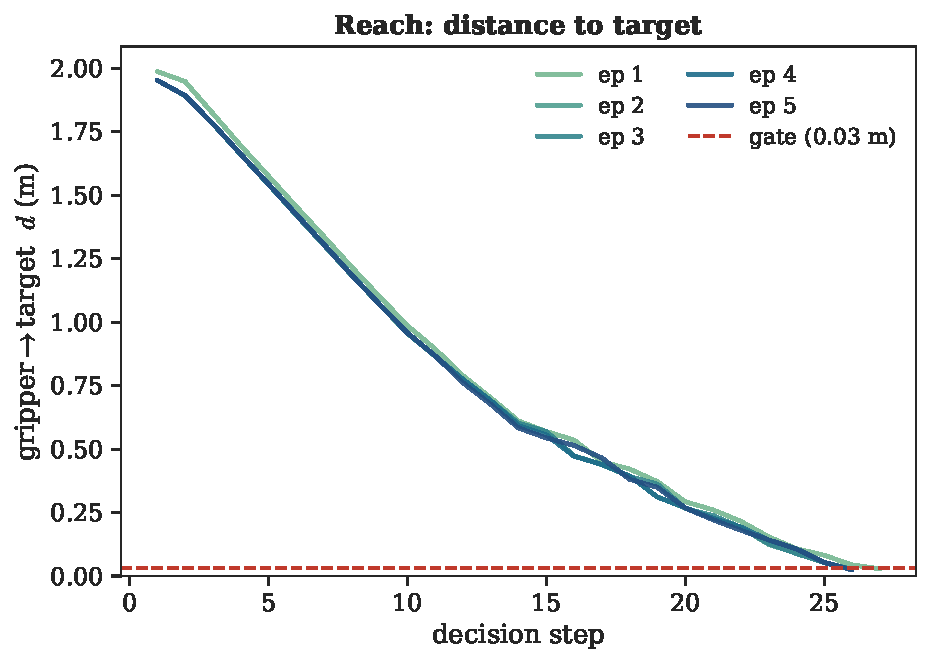
\includegraphics[width=0.80\textwidth]{s9np_reach.pdf}\end{center}
\textbf{What it shows.} Gripper$\to$target distance $d$ vs decision step, one line per episode (5 episodes); the red dashed line is the 0.03~m success gate.

\textbf{How to read it.} All 5 curves fall from $\sim$2~m to inside the gate in $\sim$26 decisions and overlap almost exactly. The target is FIXED and the policy deterministic, so the overlap is a reproducibility check.

\textbf{Say this.} ``The gripper closes from 2~m to inside the 3~cm gate in about 26 decisions, identically every episode --- deterministic and repeatable.''

\textbf{If asked.} \emph{Why do the lines overlap?} --- Fixed target + \texttt{deterministic=True} give the same trajectory each episode; the overlap confirms the run is reproducible.
\clearpage
\section*{Figure 2 --- Confondu: orientation error}
\begin{center}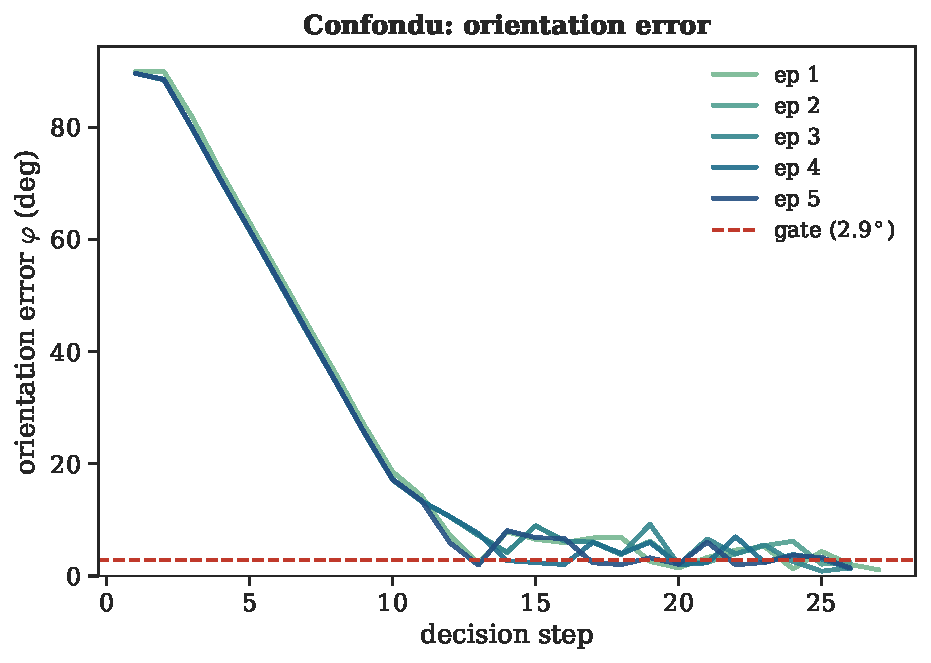
\includegraphics[width=0.80\textwidth]{s9np_orient.pdf}\end{center}
\textbf{What it shows.} Orientation error $\varphi$ (geodesic angle between the gripper frame and the target frame), in degrees, vs step; gate = 2.9$^\circ$ (0.05~rad).

\textbf{How to read it.} $\varphi$ starts near $90^\circ$ (arm home far from the target frame), drops steeply below the gate by $\sim$step 13, then holds with small residual jitter.

\textbf{Say this.} ``Orientation reaches confondu ($<2.9^\circ$) by $\sim$step 13 and holds --- the wrist aligns well before the reach finishes.''

\textbf{If asked.} \emph{What is $\varphi$?} --- the single geodesic angle between the gripper and target frames ($0$ = coincident = confondu), from the quaternion dot product $2\arccos|\langle q_G,q_T\rangle|$.
\clearpage
\section*{Figure 3 --- Base drives into arm reach}
\begin{center}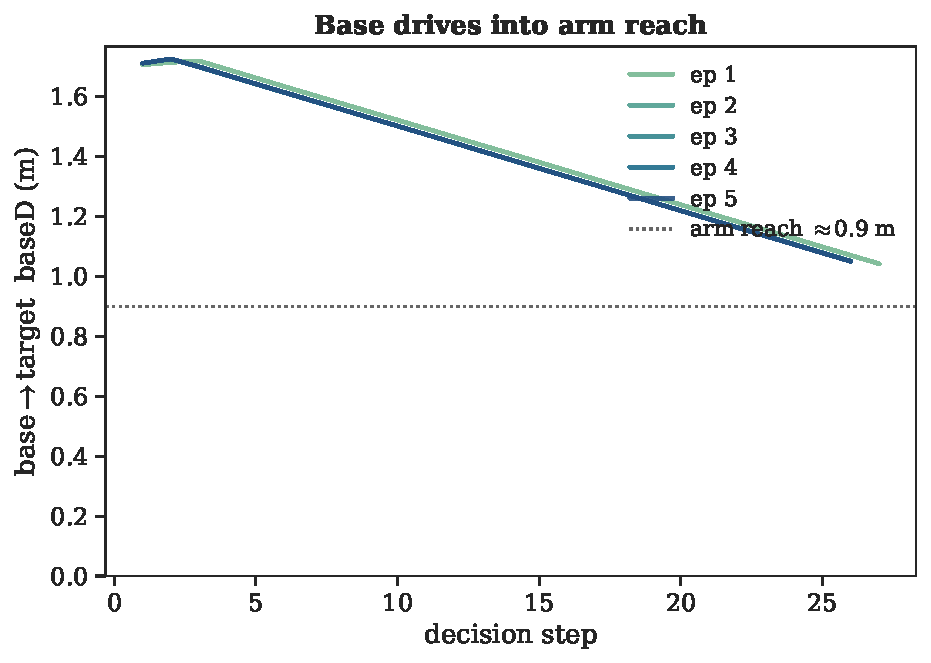
\includegraphics[width=0.80\textwidth]{s9np_basedrive.pdf}\end{center}
\textbf{What it shows.} base\_link$\to$target distance (baseD) vs step; the dotted line marks the arm reach $\approx$0.9~m.

\textbf{How to read it.} baseD falls from $\sim$1.7~m to $\sim$1.05~m --- the mobile base drives the target into the arm's working range, then the arm does the fine reach (baseD need not reach 0).

\textbf{Say this.} ``The base brings the target from 1.7~m into the arm's range, then hands off to the arm --- the whole-body division of labour.''

\textbf{If asked.} \emph{Why doesn't baseD reach 0?} --- it shouldn't; the base only has to bring the target within arm reach, the gripper (not the base) touches the target.
\clearpage
\section*{Figure 4 --- Joint convergence into the gate corner}
\begin{center}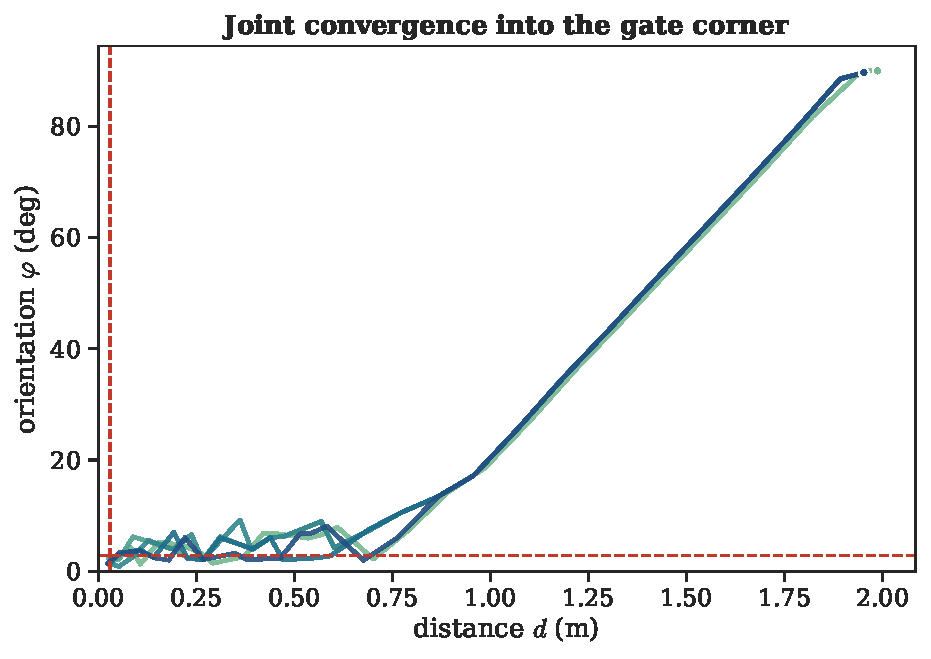
\includegraphics[width=0.80\textwidth]{s9np_phase.pdf}\end{center}
\textbf{What it shows.} The trajectory in $(d,\varphi)$ space; the dashed lines mark the gate corner ($d<0.03$~m, $\varphi<2.9^\circ$).

\textbf{How to read it.} Each run sweeps from the top-right (far, mis-oriented) into the bottom-left gate corner: $\varphi$ collapses early (by $d\approx0.8$~m), then $d$ closes the rest at low $\varphi$.

\textbf{Say this.} ``Both errors converge into the gate corner; orientation is solved first, then position closes --- a clean, non-competing convergence.''

\textbf{If asked.} \emph{Does solving orientation first cost reach time?} --- no; $\varphi$ is already under gate while $d\approx0.7$~m, so the wrist just holds alignment while the base finishes driving in.
\clearpage
\section*{Figure 5 --- Overview (one-slide summary)}
\begin{center}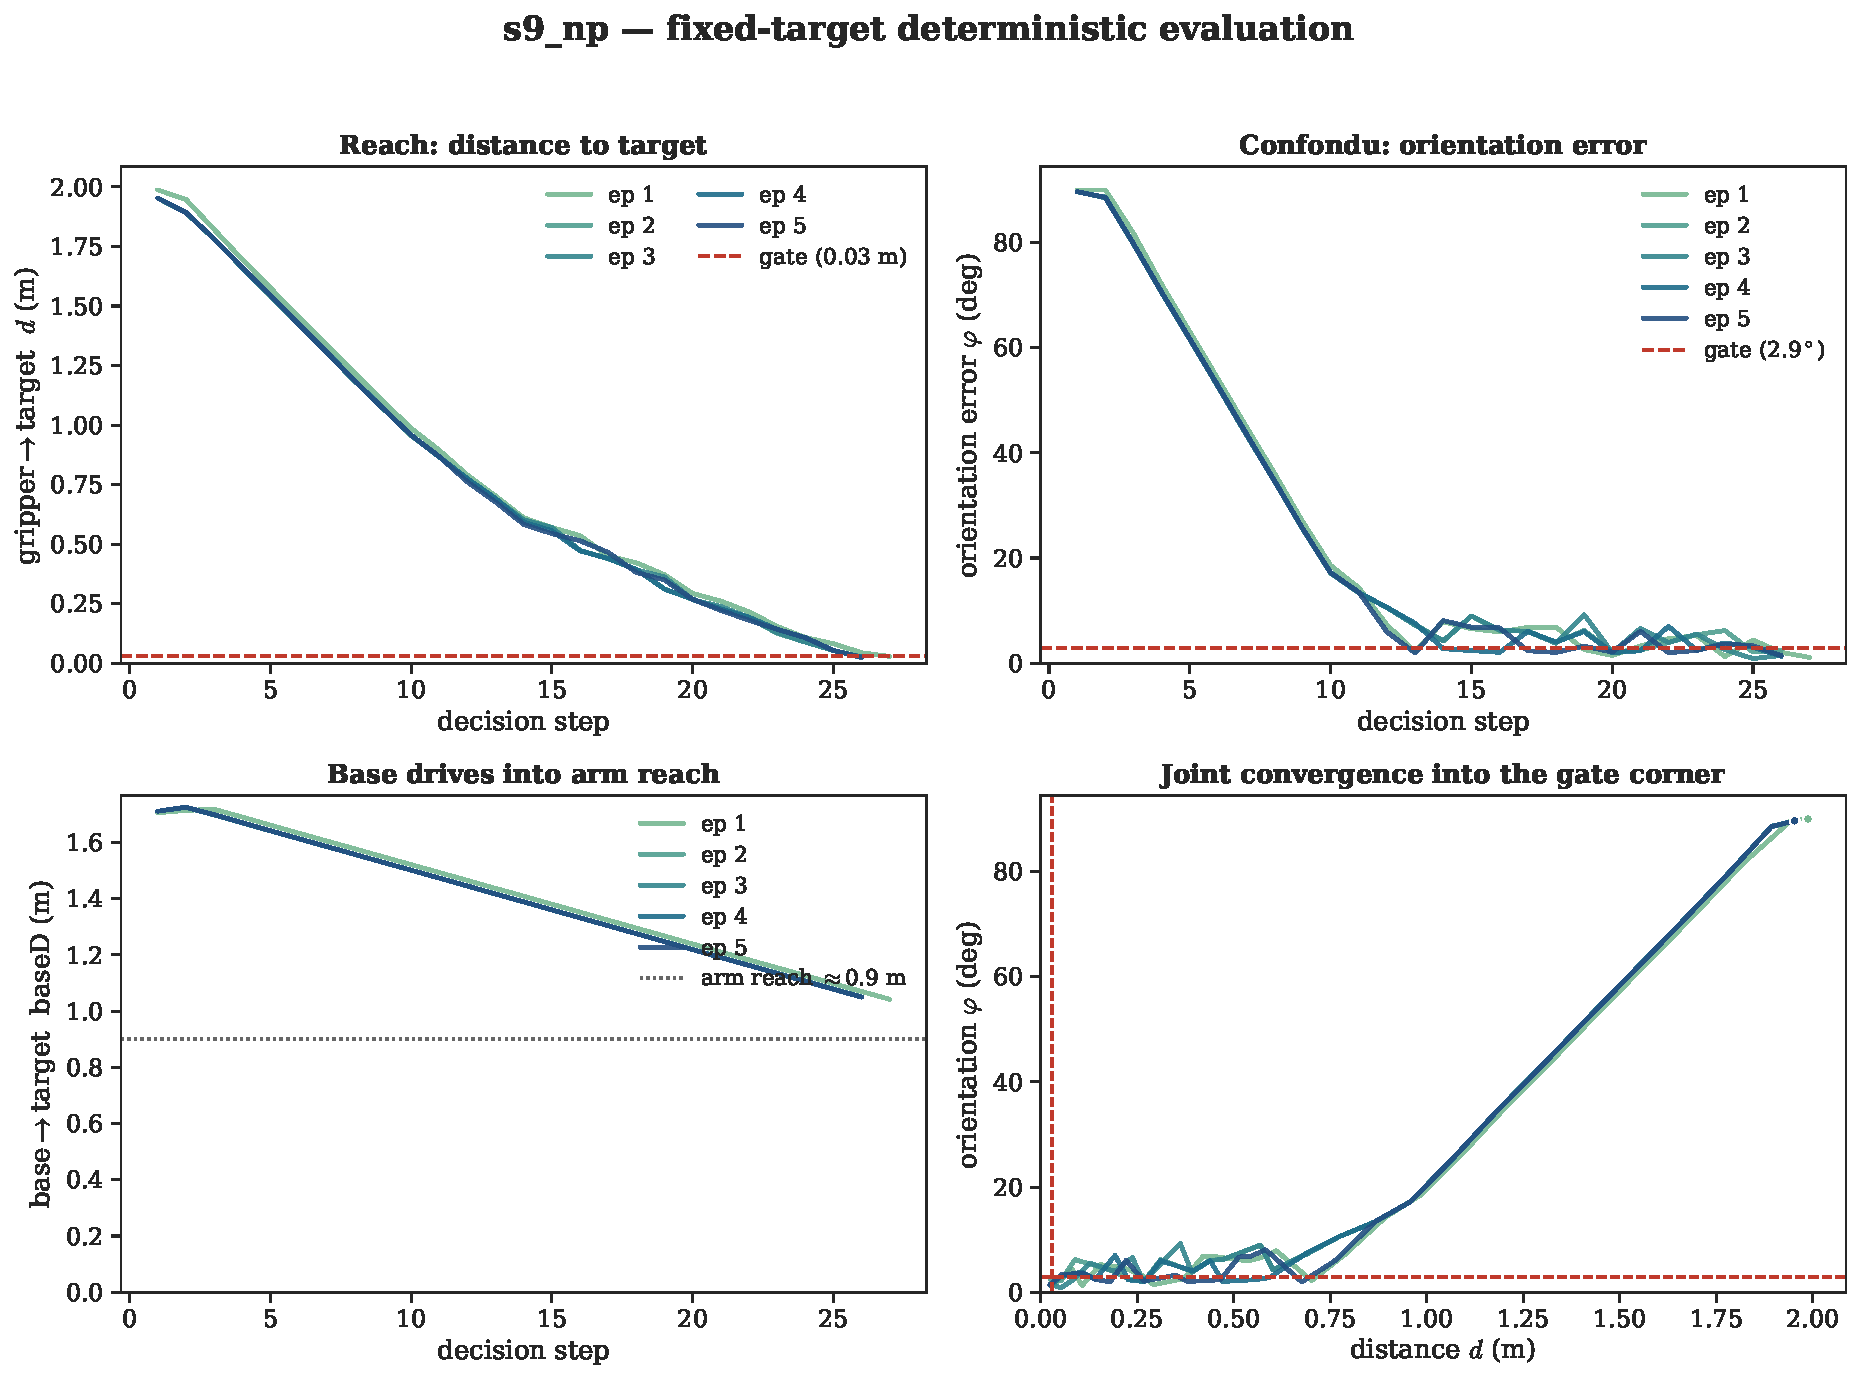
\includegraphics[width=0.80\textwidth]{s9np_overview.pdf}\end{center}
\textbf{What it shows.} The four diagnostics on one figure --- reach, orientation, base drive, and the $(d,\varphi)$ phase plot.

\textbf{How to read it.} Use as the summary slide; the panels are detailed on the preceding pages.

\textbf{Say this.} ``s9\_np reaches the 3~cm gate in $\sim$26 steps, aligns to $<2.9^\circ$, drives the base into arm range, and converges both errors into the gate corner --- 5/5 episodes, identically.''

\textbf{If asked.} \emph{One figure to remember?} --- this one: reach, confondu, base drive and joint convergence together.
\clearpage
\end{document}
